%%
%% Draft prepared from the SoftwareX OSP template.
%%

\documentclass[preprint,12pt,a4paper]{elsarticle}

\usepackage{amsmath}
\usepackage{amssymb}
\usepackage{booktabs}
\usepackage{array}
\usepackage{graphicx}
\usepackage{hyperref}
\setlength{\parindent}{0pt}
\numberwithin{equation}{section}

\journal{SoftwareX}

\begin{document}
\renewcommand{\labelenumii}{\arabic{enumi}.\arabic{enumii}}

\begin{frontmatter}

\title{AssociationProfiler: Interactive Profiling of Global and Local Conditional Associations in Mixed-Type Data}

\author[aff1]{Thadd\'ee D'haegeleer\corref{cor1}}
\ead{TODO}
\author[aff1,aff2]{C\'edric Heuchenne}
\ead{TODO}
\author[aff1,aff2]{Antoine Soetewey}
\ead{TODO}
\cortext[cor1]{Corresponding author.}
\address[aff1]{TODO: affiliation}
\address[aff2]{TODO: affiliation}

\begin{abstract}
AssociationProfiler is an open-source R Shiny application for profiling unconditional and conditional associations in multivariate datasets containing numerical and categorical variables. For every selected variable pair, the software computes a global association measure, a significance test, and local pairwise diagnostics adapted to numeric--numeric, numeric--categorical, and categorical--categorical cases. Users can filter an interactive association network with sliders for association strength and statistical significance, then inspect retained edges through harmonized unconditional or conditional pair plots. Its main contribution is the integration of partial correlations, partial eta-squared, and a Linfoot/Cox--Snell-type likelihood-ratio transformation, denoted $V_L$ and extended as $V_{L\mid Z}$, into one control-variable workflow.
\end{abstract}

\begin{keyword}
R Shiny \sep exploratory data analysis \sep association profiling \sep conditional association \sep categorical data \sep likelihood-ratio test \sep correlation network
\end{keyword}

\end{frontmatter}

\section*{Required Metadata}

\section*{Current code version}

Ancillary data table required for subversion of the codebase. The current manuscript draft refers to the GitHub repository state identified below; the final submission should replace the commit hash by a tagged release if available.

\begin{table}[!h]
\begin{tabular}{|l|p{6.5cm}|p{6.5cm}|}
\hline
\textbf{Nr.} & \textbf{Code metadata description} & \textbf{Please fill in this column} \\
\hline
C1 & Current code version & Commit \texttt{56cb1cc}; TODO: replace by release tag \\
\hline
C2 & Permanent GitHub link to code/repository used for this code version & \url{https://github.com/Thadhaeg/Partial-association-explorer} \\
\hline
C3 & Legal Code License & MIT License \\
\hline
C4 & Code versioning system used & Git/GitHub \\
\hline
C5 & Software code languages, tools, and services used & R, Shiny, bslib, dplyr, ggplot2, reactable, tidygraph, visNetwork, readxl, janitor, shinyjs, shinycssloaders, nnet, lpSolve \\
\hline
C6 & Compilation requirements, operating environments \& dependencies & R with the packages listed in the repository; tested as a local Shiny application. TODO: add R version and platform used for final validation. \\
\hline
C7 & If available Link to developer documentation/manual & TODO: repository documentation, vignette, or screencast link \\
\hline
C8 & Support email for questions & TODO \\
\hline
\end{tabular}
\caption{Code metadata (mandatory)}
\label{tab:code-metadata}
\end{table}

\section{Motivation and significance}

Many exploratory analyses start by asking which variables in a dataset are associated. In practice, this question is difficult when the dataset combines numerical variables, nominal or ordinal factors, and possible confounders. Classical correlation matrices are convenient for numerical variables but are not designed for categorical data; contingency-table measures are useful for categorical pairs but do not directly solve mixed numerical--categorical cases; and marginal pairwise summaries can be misleading when two variables are jointly related to age, education, region, time, or another background variable.

AssociationProfiler addresses this problem as a software problem rather than as a single statistical test. It provides a guided workflow for computing and visualizing both \emph{global} and \emph{local} associations between all selected pairs of variables. Global association is the single strength measure used to draw and filter the network, while a companion significance test provides a $p$-value for the corresponding null hypothesis. Users control the displayed graph with sliders for association strength and statistical significance, so the network can be tuned to highlight either strong, statistically supported patterns or weaker relationships of diagnostic interest. Local association is the observation-, group-, or cell-level diagnostic shown in the pair plots. The same app handles the unconditional case and the conditional case, where users select control variables $Z$ before recomputing the association network.

The software is intended for two audiences. For researchers, it is a fast screening tool before formal modelling: it can reveal which relationships persist after adjustment, which ones are mainly explained by controls, and which categorical cells drive a global association. For non-specialist users such as journalists, students, and data communicators, it offers a visual interface in which statistical choices are made automatically from variable types and outputs are presented with interpretable plots.

Several R packages support parts of this workflow. For numerical variables, correlation-focused packages and plotting tools provide rich correlation matrices and pairwise visual summaries. For categorical variables, classical measures such as Pearson's chi-square statistic, Cramer's $V$, information-theoretic association coefficients, and log-linear models are standard tools \cite{pearson1900,cramer1946,linfoot1957,hamdan1971,agresti2013}. AssociationExplorer, a related SoftwareX application, demonstrated how an accessible Shiny interface can lower the barrier to marginal association exploration in mixed-type data \cite{soetewey2026}. AssociationProfiler is positioned differently: it focuses on a unified \emph{association profiling} framework, likelihood-based categorical association, local diagnostics, and harmonized conditional/unconditional visual interpretation.

A central component of the categorical--categorical module is the coefficient denoted $V_L$ in the app. This notation is used for clarity within the software and should not be read as a claim that the underlying transformation is new. For two categorical variables $X$ and $Y$, the app compares a null model of independence with an alternative model allowing interaction. Let $\ell_0$ and $\ell_1$ denote the fitted log-likelihoods and let
\begin{equation}
G^2 = 2(\ell_1-\ell_0)
\label{eq:g2-intro}
\end{equation}
be the likelihood-ratio deviance. The app defines
\begin{equation}
V_L = \sqrt{1-\exp(-G^2/n)}.
\label{eq:vl-intro}
\end{equation}
In the unconditional contingency-table case, $G^2/n$ is twice the empirical mutual information between $X$ and $Y$ when natural logarithms are used. Hence $V_L=\sqrt{1-\exp[-2I(X;Y)]}$ is the sample analogue of Linfoot's informational coefficient of correlation \cite{linfoot1957}; related information measures for contingency tables were discussed by Hamdan and Tsokos \cite{hamdan1971}. The same expression is also the square root of a Cox--Snell likelihood-based coefficient of determination \cite{coxsnell1989}, related to pseudo-$R^2$ measures used in discrete-choice and generalized linear modelling \cite{mcfadden1974,nagelkerke1991}. Thus the novelty is not the unconditional transformation itself, but its use as the categorical association coefficient in an interactive conditional association workflow. It is symmetric in $X$ and $Y$, equals zero under the null model, increases monotonically with the per-observation likelihood improvement of the association model, and is built from the same likelihood-ratio statistic used for inference.

This differs from Cramer's $V$, which rescales Pearson's $\chi^2$ statistic by table dimension. Cramer's $V$ is useful for marginal contingency tables, but it is less directly tied to a nested likelihood comparison and has no single natural extension when controls include both numerical and categorical variables. Because the Linfoot/Cox--Snell transformation is likelihood-based, the app can apply the same construction in the conditional case:
\begin{equation}
V_{L\mid Z} = \sqrt{1-\exp(-G^2_{\mid Z}/n)}.
\label{eq:vlz-intro}
\end{equation}
The conditional measure therefore summarizes the residual association between $X$ and $Y$ after the separate effects of the controls have been modelled.

\section{Software description}

\subsection{Software architecture}

AssociationProfiler is a standalone Shiny application. The interface follows the analysis pipeline: data upload, variable selection, control-variable selection, association network, pair plots, and help. Users upload a CSV or Excel file and may optionally upload a two-column variable-description file. Variables with no variation are removed during preprocessing. Selected analysis variables become network nodes; selected control variables are used for adjustment but are not drawn as nodes.

\begin{figure}[!ht]
\centering
\fbox{\begin{minipage}{0.90\linewidth}
Placeholder for a workflow screenshot or schematic: data upload $\rightarrow$ variable/control selection $\rightarrow$ association computation $\rightarrow$ filtered network $\rightarrow$ pair plots.
\end{minipage}}
\caption{Planned architecture figure. The final paper should replace this placeholder by a screenshot or schematic of the app workflow.}
\label{fig:workflow}
\end{figure}

For every pair of selected variables, the backend detects the pair type and computes an association measure, a $p$-value, and a label identifying the model. The result is stored in aligned matrices used by the network and the pair-plot panel. Thresholds are applied after computation: users can filter numeric--numeric and numeric--categorical pairs by a range for $R^2$ or $\eta^2$, categorical--categorical pairs by a range for $V_L$, and all pairs by a range of $p$-values.

\subsection{Software functionalities}

\textbf{Numeric--numeric associations.} In the unconditional case, the app uses Pearson's correlation $r$ and the corresponding $R^2=r^2$ for thresholding. In the conditional case, it uses the added-variable principle: $X$ and $Y$ are separately regressed on the controls $Z$, and the association is the correlation between the residuals. The pair plot is harmonized across cases: raw scatter plots are used without controls, and residual scatter plots are used with controls. Both show the fitted linear trend and can have their axes reversed.

\textbf{Numeric--categorical associations.} For a numerical variable $Y$ and a categorical variable $X$, the unconditional measure is the ANOVA effect size
\begin{equation}
\eta^2=\frac{\mathrm{SSB}}{\mathrm{SST}},
\label{eq:eta2-main}
\end{equation}
the proportion of variance in $Y$ explained by differences between group means. This is more appropriate than applying Pearson correlation to arbitrary numeric encodings of categories. In the conditional case, the app uses an ANCOVA/extra-sum-of-squares construction. It compares a reduced model $Y\sim Z$ to a full model $Y\sim X+Z$ and reports
\begin{equation}
\eta^2_{X\mid Z}=
\frac{\mathrm{RSS}_{red}-\mathrm{RSS}_{full}}
{\mathrm{RSS}_{red}-\mathrm{RSS}_{full}+\mathrm{RSS}_{full}}.
\label{eq:eta2z-main}
\end{equation}
The corresponding $F$-test provides the global $p$-value. The pair plots are again harmonized: unconditional plots display group means of $Y$ by $X$, while conditional plots display group means of the residualized outcome $Y-\widehat{E}(Y\mid Z)$. Thus the visual object remains a mean plot, but the quantity being averaged changes from raw values to adjusted residuals.

\textbf{Categorical--categorical associations.} The categorical--categorical module treats the pair $(X,Y)$ as a single joint multinomial outcome $W=(X,Y)$ with $I J$ possible categories and fits baseline-category multinomial logits relative to the first cell. Under the null model,
\begin{equation}
\eta^{(0)}_{ij}(z)=\alpha_i+\beta_j+\lambda_i^\top z+\kappa_j^\top z,
\label{eq:eta0-main}
\end{equation}
whereas the alternative model adds an interaction block
\begin{equation}
\eta^{(1)}_{ij}(z)=\eta^{(0)}_{ij}(z)+\gamma_{ij}.
\label{eq:eta1-main}
\end{equation}
Identifiability is enforced through reference-category constraints:
\begin{equation}
\alpha_1=\beta_1=0,\qquad
\lambda_1=\mathbf{0},\qquad
\kappa_1=\mathbf{0},\qquad
\gamma_{1j}=\gamma_{i1}=0.
\label{eq:constraints-main}
\end{equation}
For $m\in\{0,1\}$, the corresponding probabilities are
\begin{equation}
\pi^{(m)}_{ij}(z;\theta)=
\frac{\exp\!\left(\eta^{(m)}_{ij}(z)\right)}
{\sum_{r=1}^{I}\sum_{s=1}^{J}\exp\!\left(\eta^{(m)}_{rs}(z)\right)},
\label{eq:pi-main}
\end{equation}
with the baseline cell receiving linear predictor zero. The app maximizes the log-likelihood
\begin{equation}
\ell_m(\theta)=
\sum_{t=1}^{n}\sum_{i=1}^{I}\sum_{j=1}^{J}
\mathbf{1}\{X_t=i,Y_t=j\}\log \pi^{(m)}_{ij}(Z_t;\theta),
\qquad m\in\{0,1\},
\label{eq:loglik-main}
\end{equation}
using a BFGS optimizer with analytic gradients; repeated control-design rows are grouped internally for efficiency, but the criterion is algebraically the same as \eqref{eq:loglik-main}. The fitted null model produces expected counts
\begin{equation}
E^{(0)}_{ij}=
\sum_{t=1}^{n}\Pr(X=i,Y=j\mid Z_t;\widehat{\theta}_0)
=
\sum_{t=1}^{n}\pi^{(0)}_{ij}(Z_t;\widehat{\theta}_0),
\label{eq:e0-main}
\end{equation}
which reduce to the classical independence expectations in the unconditional contingency-table case.

This design was chosen after considering Poisson log-linear alternatives. For ordinary contingency tables, Poisson log-linear models are elegant and standard \cite{agresti2013,nelder1972}. With categorical controls, a multiway table can also represent conditional independence. However, this approach becomes fragile in an interactive app when controls may be continuous or numerous: continuous controls must be discretized, arbitrary bins create modelling choices, and multiway tables rapidly become sparse. The structured multinomial likelihood avoids these difficulties by using controls as regression covariates, after model-matrix coding for categorical controls, while preserving a nested likelihood-ratio comparison between a null and an interaction model.

\textbf{Local categorical diagnostics.} For categorical pairs, the app computes both the observed-minus-expected deviation
\begin{equation}
D_{ij}=O_{ij}-E^{(0)}_{ij}
\label{eq:dij-main}
\end{equation}
and the Pearson residual
\begin{equation}
R_{ij}=\frac{O_{ij}-E^{(0)}_{ij}}{\sqrt{E^{(0)}_{ij}}}.
\label{eq:rij-main}
\end{equation}
In the current app, the categorical pair plot displays $R_{ij}$ directly inside each cell and also uses $R_{ij}$ for the colour scale: positive residuals are shown in red, negative residuals in blue, and darker shades indicate larger standardized departures from the null model. The same display grammar is used with and without controls; only the expected counts $E^{(0)}_{ij}$ change.

\begin{figure}[!ht]
\centering
\fbox{\begin{minipage}{0.90\linewidth}
Placeholder for three pair-plot screenshots: scatter/residual scatter, group means/residualized means, and categorical residual table.
\end{minipage}}
\caption{Planned pair-plot figure. The final paper should show one example for each variable-type case and, ideally, include conditional and unconditional versions side by side.}
\label{fig:pairplots}
\end{figure}

\textbf{Optimal submatrix display for large categorical tables.} Large contingency tables are difficult to read in a browser. The current app displays the full table as long as the number of cells does not exceed $49$. Beyond that threshold, it selects a submatrix with at most $7$ rows and $7$ columns. The selection score is not the raw likelihood-ratio contribution but the squared Pearson residual,
\begin{equation}
S_{ij}=R_{ij}^2=\frac{\left(O_{ij}-E^{(0)}_{ij}\right)^2}{E^{(0)}_{ij}},
\label{eq:score-main}
\end{equation}
which is nonnegative and directly aligned with the residual-based visual encoding used in the pair plot. If at most $m_r=\min(I,7)$ rows and $m_c=\min(J,7)$ columns can be shown, the app solves
\begin{equation}
\max_{u,v,z}\sum_{i=1}^{I}\sum_{j=1}^{J} S_{ij}z_{ij},
\label{eq:sub-obj-main}
\end{equation}
subject to
\begin{align}
\sum_{i=1}^{I}u_i &= m_r,
&
\sum_{j=1}^{J}v_j &= m_c,
\label{eq:sub-cons-main-a}
\\
z_{ij} &\le u_i,
&
z_{ij} &\le v_j,
\label{eq:sub-cons-main-b}
\\
z_{ij} &\ge u_i+v_j-1.
\label{eq:sub-cons-main-c}
\end{align}
Here $u_i$ and $v_j$ indicate selected rows and columns, and $z_{ij}$ indicates that cell $(i,j)$ is displayed. The implementation uses \texttt{lpSolve} when available and otherwise falls back to a heuristic based on the largest scores $S_{ij}$. The app also reports the proportion of total score retained by the displayed submatrix.

\subsection{Sample code snippets analysis}

The following simplified code illustrates the current submatrix selection logic. It is included because this feature connects the residual-based local diagnostics to the interface design.

\begin{verbatim}
compute_display_scores <- function(O, E0) {
  S <- matrix(0, nrow = nrow(O), ncol = ncol(O))
  ok <- is.finite(E0) & (E0 > 0)
  S[ok] <- ((O[ok] - E0[ok])^2) / E0[ok]
  S[!is.finite(S) | S < 0] <- 0
  S
}

select_catcat_display_submatrix <- function(S, max_dim = 7L) {
  if ((nrow(S) * ncol(S)) <= (max_dim * max_dim))
    return(list(rows = seq_len(nrow(S)),
                cols = seq_len(ncol(S)),
                reduced = FALSE))
  find_optimal_submatrix(S, n = max_dim)
}
\end{verbatim}

This code makes explicit that the displayed categories are chosen from the same standardized residual structure that is ultimately shown to the user.

\section{Illustrative example: age as a confounder of the health--internet-use association}

Imagine a user exploring a Belgian extract of the European Social Survey and wanting a first overview of how everyday behaviours and attitudes are connected. They select five categorical variables in the app: frequency of internet use (\texttt{netusoft}), received at least one COVID-19 vaccine (\texttt{vacc19}), subjective general health (\texttt{health}), alcohol consumption (\texttt{alcfreq}), and attendance at religious services (\texttt{rlgatnd}). At this stage the goal is exploratory rather than confirmatory: the user wants to see which links are strong enough to deserve closer inspection and which ones may disappear once an obvious background factor is taken into account.

The thresholds are set to the values shown in the screenshots: a lower bound of 0.1 for both the quantitative/mixed slider and the categorical slider, and a $p$-value range from 0 to 0.05. This is a reasonable compromise for an exploratory pass. The effect-size threshold removes very small associations that would clutter the graph, while the $p$-value threshold keeps the focus on links that are still statistically supported at a conventional level. In other words, the network is not meant to display every detectable relation in the data, but the subset that is both non-negligible and significant enough to be worth discussing.

\begin{figure}[!ht]
\centering
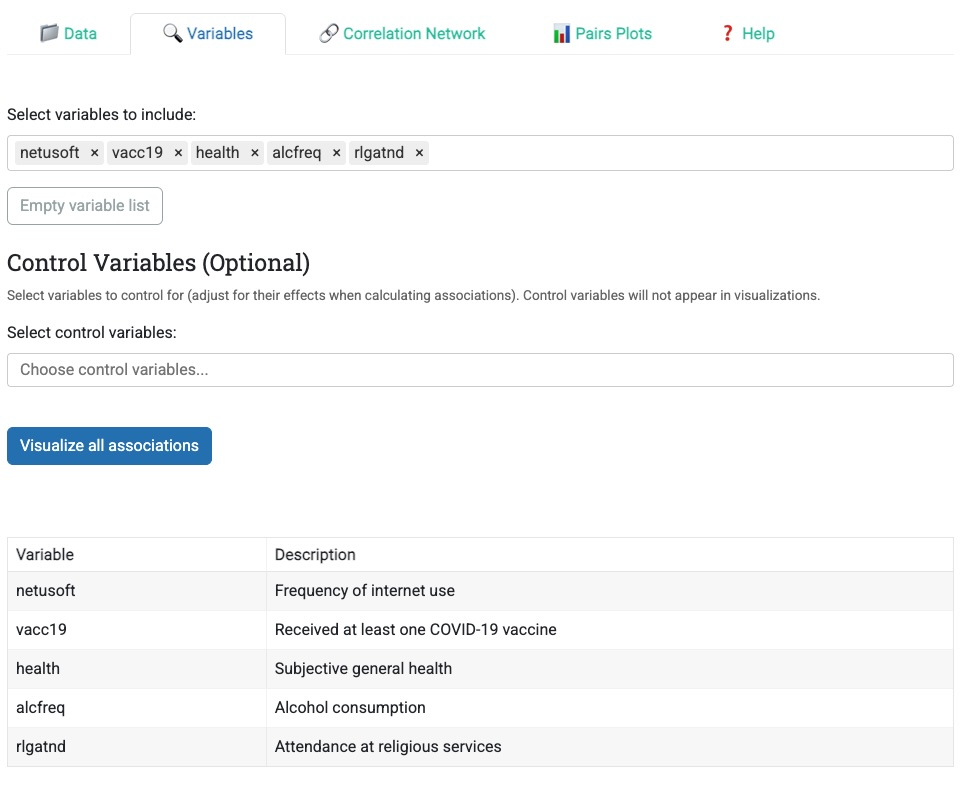
\includegraphics[width=0.82\linewidth]{variables_selection.jpg}
\par\medskip
\begin{minipage}{0.48\linewidth}
\centering
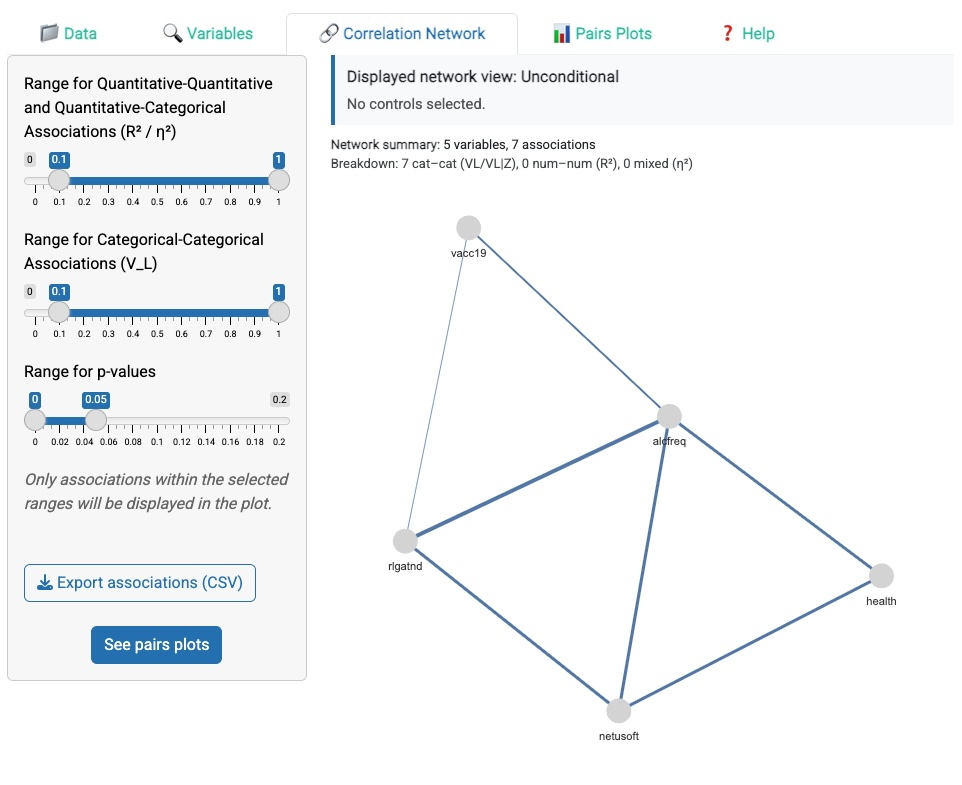
\includegraphics[width=\linewidth]{uncond_network.jpg}
\par\smallskip
\small (a) Unconditional association network.
\end{minipage}
\hfill
\begin{minipage}{0.48\linewidth}
\centering
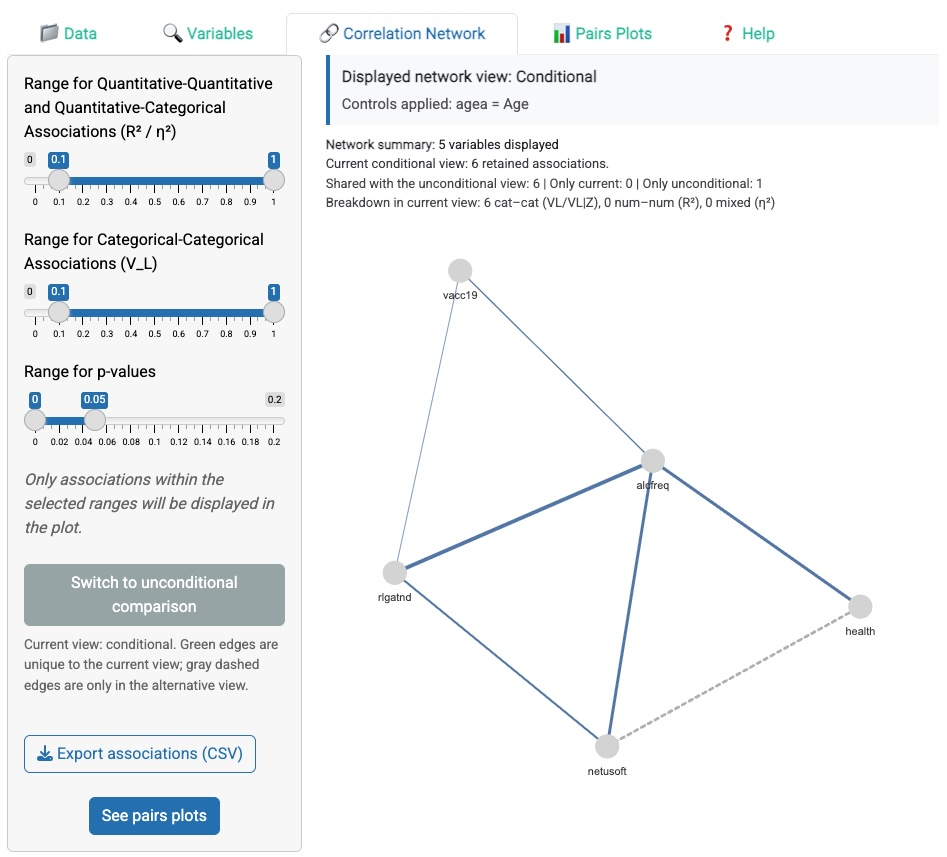
\includegraphics[width=\linewidth]{cond_network.jpg}
\par\smallskip
\small (b) Conditional association network with \texttt{agea} as control.
\end{minipage}
\caption{Illustrative workflow. Top: selected analysis variables in the app. Bottom-left: unconditional network. Bottom-right: conditional network after controlling for age. In this example, the \texttt{health}--\texttt{netusoft} edge is retained without controls but disappears after conditioning on age.}
\label{fig:network-example}
\end{figure}

Figure~\ref{fig:network-example} shows the first two steps of this exploration. Without controls, the network retains seven associations among the five variables, all of them categorical--categorical. One of the retained edges links \texttt{health} and \texttt{netusoft}. This edge is immediately interesting in substantive terms: it suggests that self-rated health and internet use are related in the raw data, but it does not yet tell us whether the relationship is direct or whether it is partly produced by some third variable that shapes both.

The next step is to open the pair plot for this edge. The unconditional table in Figure~\ref{fig:uncond-pairplot} makes the direction of the association much clearer. Respondents who never use the internet are under-represented in the \emph{very good} health category and strongly over-represented in the \emph{fair} and \emph{very bad} categories. At the other end of the scale, respondents who use the internet every day are over-represented in \emph{very good} health and under-represented in \emph{fair} or \emph{very bad} health. Read as a whole, the table suggests a simple marginal story: more frequent internet use is associated with better self-rated health.

\begin{figure}[!ht]
\centering
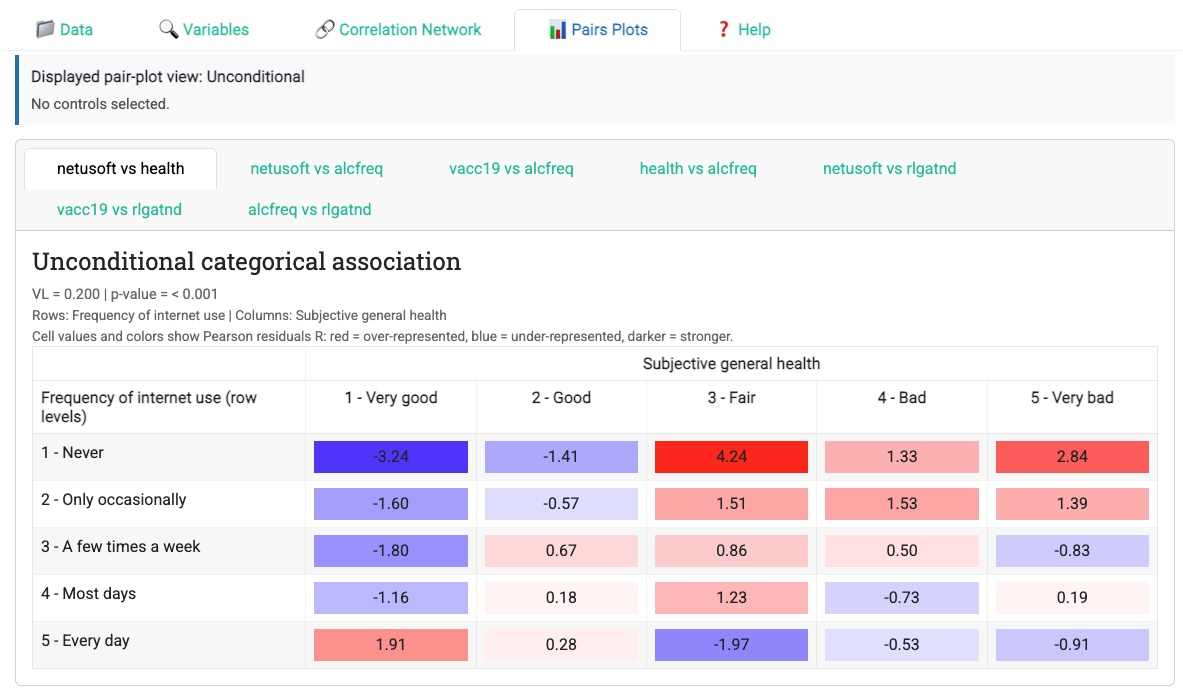
\includegraphics[width=0.92\linewidth]{uncond_pairplot.jpg}
\caption{Unconditional pair plot for \texttt{netusoft} and \texttt{health}. The Pearson-residual colours and values show that low internet use is associated with worse self-rated health in the raw data, whereas daily internet use is associated with better self-rated health.}
\label{fig:uncond-pairplot}
\end{figure}

However, this is exactly the kind of pattern for which a user may suspect confounding. Age is a natural candidate: older respondents tend to report worse health and also to use the internet less frequently. If both variables are strongly age-graded, then the unconditional association between \texttt{health} and \texttt{netusoft} may be real as a marginal fact but misleading as a direct relationship. The same reasoning could apply to other edges in the network as well, which is why the app allows the user to select control variables and recompute the whole structure rather than inspecting each pair separately by hand.

The user therefore adds age (\texttt{agea}) as a control and reruns the analysis. The conditional network in Figure~\ref{fig:network-example} now retains six associations instead of seven. The edge between \texttt{health} and \texttt{netusoft} disappears from the retained conditional graph and is shown only as a dashed unconditional-only edge in the comparison view. This is already a strong visual clue that the original relationship was largely driven by age.

\begin{figure}[!ht]
\centering
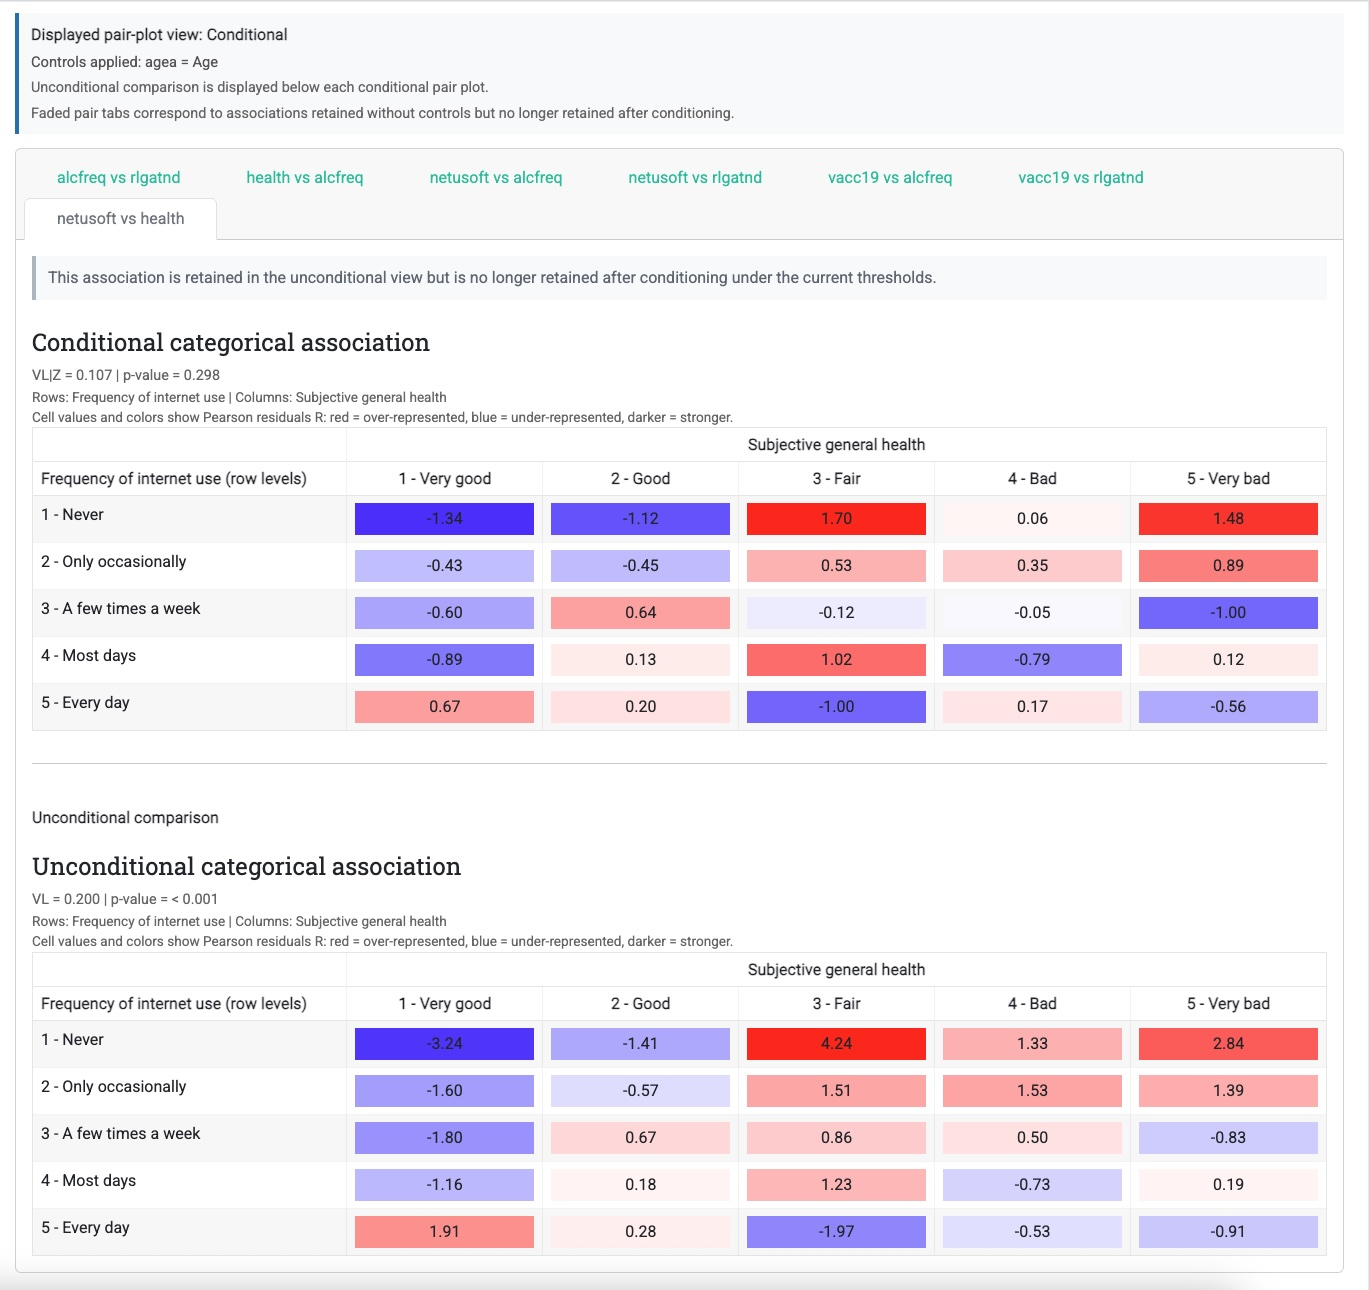
\includegraphics[width=0.96\linewidth]{pair_plots.jpg}
\caption{Conditional and unconditional pair plots for \texttt{netusoft} versus \texttt{health} after adding \texttt{agea} as control. The conditional tab is kept visible even though the edge is no longer retained after adjustment, and the unconditional comparison is shown below it.}
\label{fig:pairplots-example}
\end{figure}

Figure~\ref{fig:pairplots-example} explains the change more formally. Because both variables are categorical, the app reports $V_L$ in the unconditional case and $V_{L\mid Z}$ in the conditional case. Without controls, the association is moderate and statistically significant ($V_L = 0.200$, $p < 0.001$). After conditioning on age, it drops to $V_{L\mid Z} = 0.107$ with $p = 0.298$, so the null hypothesis of conditional independence is no longer rejected at the chosen threshold.

The local tables tell the same story. After controlling for age, the most pronounced residual deviations become smaller: the cells that combined no internet use with worse health are still somewhat positive, but much less so than in the raw table, and the contrast with daily internet users becomes less sharp. The conditional table therefore no longer supports the strong gradient seen in the unconditional view. In substantive terms, much of the original health--internet-use association seems to reflect the fact that older respondents are both less connected digitally and more likely to report worse health.

This small example captures the intended use of AssociationProfiler. A user starts with a readable network filtered to non-negligible and significant edges, identifies a substantively interesting link, inspects its local direction in the pair plot, and then asks whether a plausible third variable could be generating the pattern. By introducing age as a control, the app turns a simple descriptive association into a more informative story about confounding. In that sense, the software is not only a visualization tool but also a practical guide for moving from marginal patterns to adjusted interpretation in mixed-type data.

\section{Impact}

AssociationProfiler enables exploratory questions that are difficult to ask with standard pairwise tools. Instead of asking only whether two variables are marginally associated, users can ask whether the association remains after controlling for selected background variables. This supports more careful screening in survey analysis, public-data exploration, education, and preliminary research workflows.

The software improves existing exploratory practice in four ways. First, it unifies association measures for all common pair types in a single interface. Second, it makes conditional association analysis accessible without requiring users to write regression, ANOVA, or multinomial likelihood code. Third, it combines effect-size filtering with formal significance tests, allowing users to tune the network with strength and $p$-value sliders rather than relying on a single threshold. Fourth, it connects global network edges to local diagnostics so users can inspect the pattern behind each association. This is particularly important for categorical data, where a global statistic may be driven by a small number of over- or under-represented cells.

The likelihood-based categorical module is expected to be useful beyond the immediate Shiny app. The notation $V_L$ makes an established Linfoot/Cox--Snell transformation explicit in the app, while $V_{L\mid Z}$ applies the same transformation to a conditional likelihood-ratio comparison. The conditional version allows numerical and categorical controls to enter the same framework, avoiding the need to discretize continuous controls into multiway contingency tables. This creates a natural bridge between contingency-table exploration and model-based exploratory analysis.

For non-specialist users, the impact lies in making cautious data exploration easier. Journalists and data communicators often work with public datasets containing mixed variable types and many plausible confounders. The app can help identify associations worth investigating further while making the distinction between marginal and adjusted patterns visible. For researchers and students, the app can serve as a teaching and diagnostic tool for partial correlation, ANCOVA, likelihood-ratio testing, pseudo-$R^2$ measures, and conditional independence.

The software is not intended to establish causal effects. Conditional associations depend on the selected controls and on the adequacy of the working models. Sparse categorical tables, rare categories, separation-like behaviour in multinomial fitting, and misspecified control effects may affect the reliability of both global and local summaries. The app is therefore best understood as a transparent exploratory layer that helps users decide where more formal modelling is warranted.

\section{Conclusions}

AssociationProfiler is an open-source Shiny application for global and local association exploration in mixed-type datasets. It provides unconditional and conditional association measures for numeric--numeric, numeric--categorical, and categorical--categorical pairs; filters the resulting network by effect size and statistical significance; and displays harmonized pair plots that explain the local structure of retained associations.

The main novelties are the integrated control-variable workflow, the extension of an established Linfoot/Cox--Snell-type categorical association coefficient to conditional association through $V_{L\mid Z}$, the structured multinomial approach for categorical pairs with numerical or categorical controls, residualized pair plots for conditional interpretation, and the optimal submatrix display for large contingency tables.

\section*{Acknowledgements}

TODO: Add funding, project acknowledgements, institutional acknowledgements, and thanks to testers or contributors.

\appendix

\section{Additional mathematical details for the categorical--categorical module}

This appendix records the likelihood specification used by the current app implementation more explicitly than in the main text.

Let $W=(X,Y)$ denote the joint outcome, with $X$ having $I$ levels and $Y$ having $J$ levels. Then $W$ has $K=IJ$ possible categories. The app uses baseline-category multinomial logits with the first level of $X$ and the first level of $Y$ as reference categories.

\subsection{Unconditional case}

For the unconditional analysis, the null and alternative predictors are
\begin{align}
\eta^{(0)}_{ij} &= \alpha_i + \beta_j,
\label{eq:app-uncond-null}
\\
\eta^{(1)}_{ij} &= \alpha_i + \beta_j + \gamma_{ij},
\label{eq:app-uncond-alt}
\end{align}
with $\alpha_1=\beta_1=0$ and $\gamma_{1j}=\gamma_{i1}=0$. The corresponding probabilities are
\begin{equation}
\pi^{(m)}_{ij}(\theta)=
\frac{\exp\!\left(\eta^{(m)}_{ij}\right)}
{\sum_{r=1}^{I}\sum_{s=1}^{J}\exp\!\left(\eta^{(m)}_{rs}\right)},
\qquad m\in\{0,1\}.
\label{eq:app-uncond-prob}
\end{equation}

If $O_{ij}$ denotes the observed contingency-table counts, the maximized log-likelihoods used to compute $V_L$ are
\begin{equation}
\ell_m(\theta)=
\sum_{i=1}^{I}\sum_{j=1}^{J}
O_{ij}\log \pi^{(m)}_{ij}(\theta),
\qquad m\in\{0,1\}.
\label{eq:app-uncond-loglik}
\end{equation}

The null-model expected counts are then
\begin{equation}
E^{(0)}_{ij}=n\,\pi^{(0)}_{ij}(\widehat{\theta}_0),
\label{eq:app-uncond-expected}
\end{equation}
which coincide with the classical independence expectations. In the code, a direct independence fallback based on row and column marginals is also available if the null optimization fails.

\subsection{Conditional case}

When controls $Z$ are present, the app first converts them into a regression design matrix. Numerical controls are kept as they are; categorical controls are represented by their model-matrix coding. If several observations share the same coded control vector, they are grouped before optimization. Let $z^{(g)}$, $g=1,\dots,G$, denote the distinct design rows and let $N_{gij}$ be the number of observations in joint category $(i,j)$ within group $g$.

The null and alternative predictors become
\begin{align}
\eta^{(0)}_{ij}(z)
&=
\alpha_i+\beta_j+\lambda_i^\top z+\kappa_j^\top z,
\label{eq:app-cond-null}
\\
\eta^{(1)}_{ij}(z)
&=
\alpha_i+\beta_j+\lambda_i^\top z+\kappa_j^\top z+\gamma_{ij},
\label{eq:app-cond-alt}
\end{align}
with constraints
\begin{align}
\alpha_1 &= 0,
&
\beta_1 &= 0,
\label{eq:app-cond-cons-a}
\\
\lambda_1 &= \mathbf{0},
&
\kappa_1 &= \mathbf{0},
\label{eq:app-cond-cons-b}
\\
\gamma_{1j} &= 0 \quad \text{for all } j,
&
\gamma_{i1} &= 0 \quad \text{for all } i.
\label{eq:app-cond-cons-c}
\end{align}

The grouped conditional log-likelihood maximized by the app is
\begin{equation}
\ell_m(\theta)=
\sum_{g=1}^{G}\sum_{i=1}^{I}\sum_{j=1}^{J}
N_{gij}\log \pi^{(m)}_{ij}(z^{(g)};\theta),
\qquad m\in\{0,1\},
\label{eq:app-cond-loglik-grouped}
\end{equation}
which is algebraically equivalent to the observation-level form in Equation~\eqref{eq:loglik-main}. This grouped representation is the reason the current implementation remains much faster than a naive observation-by-observation likelihood evaluation when many rows share the same control pattern.

The null-model expected counts displayed in the pair plots are
\begin{equation}
E^{(0)}_{ij}
=
\sum_{g=1}^{G} n_g\,\pi^{(0)}_{ij}(z^{(g)};\widehat{\theta}_0)
=
\sum_{t=1}^{n}\pi^{(0)}_{ij}(Z_t;\widehat{\theta}_0),
\label{eq:app-cond-expected}
\end{equation}
where $n_g=\sum_{i,j}N_{gij}$ is the size of group $g$. The global likelihood-ratio statistic uses the same degrees of freedom in the unconditional and conditional cases,
\begin{equation}
\mathrm{df}=(I-1)(J-1),
\label{eq:app-df}
\end{equation}
because only the interaction block differs between the null and alternative models.

In the current implementation, both models are fit with BFGS through \texttt{optim()}, using an analytic gradient. The alternative model is warm-started from the null-model estimate by adding zero-valued interaction parameters before optimization.

\section{Local diagnostics and optimal submatrix display}

The app computes two local quantities for each cell:
\begin{align}
D_{ij} &= O_{ij}-E^{(0)}_{ij},
\label{eq:app-dij}
\\
R_{ij} &= \frac{O_{ij}-E^{(0)}_{ij}}{\sqrt{E^{(0)}_{ij}}}.
\label{eq:app-rij}
\end{align}
Both are stored internally, but the current categorical pair plots display only $R_{ij}$ as the printed cell value. The colour scale is also driven by $R_{ij}$, so the sign and magnitude shown visually are exactly the sign and magnitude of the Pearson residual. Positive cells are over-represented relative to the fitted null model, negative cells are under-represented, and darker colours indicate larger standardized departures.

For large tables, the app does not optimize on raw deviance contributions. Instead it builds the nonnegative score matrix
\begin{equation}
S_{ij}=R_{ij}^2=\frac{\left(O_{ij}-E^{(0)}_{ij}\right)^2}{E^{(0)}_{ij}},
\label{eq:app-score}
\end{equation}
which coincides with the cellwise Pearson chi-square contribution. If the table has at most $49$ cells, the full table is shown. Otherwise the app selects at most seven rows and seven columns by solving the binary program in Equations~\eqref{eq:sub-obj-main}--\eqref{eq:sub-cons-main-c}. The exact optimization is used when \texttt{lpSolve} is available; otherwise the app falls back to a heuristic that keeps the rows and columns appearing most often among the largest positive scores.

Finally, when a reduced table is shown, the app reports the coverage rate
\begin{equation}
\mathrm{Coverage}=
\frac{\sum_{(i,j)\in\mathcal{S}} S_{ij}}
{\sum_{i=1}^{I}\sum_{j=1}^{J} S_{ij}},
\label{eq:app-coverage}
\end{equation}
where $\mathcal{S}$ denotes the selected submatrix. This percentage tells the user how much of the residual structure is still visible after the display has been trimmed to a manageable size.

\begin{thebibliography}{00}

\bibitem{pearson1900}
K. Pearson, On the criterion that a given system of deviations from the probable in the case of a correlated system of variables is such that it can be reasonably supposed to have arisen from random sampling, Philosophical Magazine 50 (1900) 157--175.

\bibitem{cramer1946}
H. Cram\'er, Mathematical Methods of Statistics, Princeton University Press, Princeton, 1946.

\bibitem{linfoot1957}
E.H. Linfoot, An informational measure of correlation, Information and Control 1 (1) (1957) 85--89. \url{https://doi.org/10.1016/S0019-9958(57)90116-X}

\bibitem{hamdan1971}
M.A. Hamdan, C.P. Tsokos, An information measure of association in contingency tables, Information and Control 19 (2) (1971) 174--179. \url{https://doi.org/10.1016/S0019-9958(71)90799-6}

\bibitem{agresti2013}
A. Agresti, Categorical Data Analysis, 3rd ed., Wiley, Hoboken, 2013.

\bibitem{coxsnell1989}
D.R. Cox, E.J. Snell, Analysis of Binary Data, 2nd ed., Chapman and Hall, London, 1989.

\bibitem{mcfadden1974}
D. McFadden, Conditional logit analysis of qualitative choice behavior, in: P. Zarembka (Ed.), Frontiers in Econometrics, Academic Press, New York, 1974, pp. 105--142.

\bibitem{nagelkerke1991}
N.J.D. Nagelkerke, A note on a general definition of the coefficient of determination, Biometrika 78 (3) (1991) 691--692. \url{https://doi.org/10.1093/biomet/78.3.691}

\bibitem{nelder1972}
J.A. Nelder, R.W.M. Wedderburn, Generalized linear models, Journal of the Royal Statistical Society: Series A 135 (3) (1972) 370--384.

\bibitem{cohen1973}
J. Cohen, Eta-squared and partial eta-squared in fixed factor ANOVA designs, Educational and Psychological Measurement 33 (1973) 107--112.

\bibitem{levine2002}
T.R. Levine, C.R. Hullett, Eta squared, partial eta squared, and misreporting of effect size in communication research, Human Communication Research 28 (4) (2002) 612--625.

\bibitem{soetewey2026}
A. Soetewey, C. Heuchenne, A. Claes, A. Descampe, AssociationExplorer: A user-friendly Shiny application for exploring associations and visual patterns, SoftwareX 33 (2026) 102483. \url{https://doi.org/10.1016/j.softx.2025.102483}

\bibitem{r}
R Core Team, R: A language and environment for statistical computing, R Foundation for Statistical Computing, Vienna, Austria, 2024. \url{https://www.R-project.org/}

\bibitem{shiny}
W. Chang, J. Cheng, J.J. Allaire, C. Sievert, B. Schloerke, Y. Xie, J. Allen, J. McPherson, A. Dipert, B. Borges, shiny: Web application framework for R, R package, 2024. \url{https://CRAN.R-project.org/package=shiny}

\bibitem{visnetwork}
Almende B.V. and contributors, B. Thieurmel, visNetwork: Network visualization using vis.js library, R package, 2022. \url{https://CRAN.R-project.org/package=visNetwork}

\bibitem{lpsolve}
M. Berkelaar, lpSolve: Interface to Lp\_solve v. 5.5 to solve linear/integer programs, R package. \url{https://CRAN.R-project.org/package=lpSolve}

\end{thebibliography}

\section*{Current executable software version}

\begin{table}[!h]
\begin{tabular}{|l|p{6.5cm}|p{6.5cm}|}
\hline
\textbf{Nr.} & \textbf{Executable software metadata description} & \textbf{Please fill in this column} \\
\hline
S1 & Current software version & Commit \texttt{56cb1cc}; TODO: replace by release tag \\
\hline
S2 & Permanent link to executable software of this version & \url{https://github.com/Thadhaeg/Partial-association-explorer} \\
\hline
S3 & Legal Software License & MIT License \\
\hline
S4 & Computing platforms/Operating Systems & Platform independent where R and package dependencies are available; TODO: tested OS list \\
\hline
S5 & Installation requirements \& dependencies & Install R and packages listed in the repository; run the Shiny application from \texttt{app.r}. TODO: add exact installation command or renv lockfile. \\
\hline
\end{tabular}
\caption{Software metadata (optional executable version table)}
\label{tab:software-metadata}
\end{table}

\end{document}
